\documentclass[border=5mm, varwidth]{standalone}
\usepackage{tikz}
\begin{document}

\begin{tabular}{@{}c@{}}

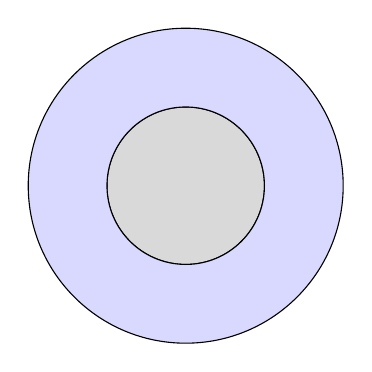
\begin{tikzpicture}
\filldraw [fill=gray!30, draw=black] (0,0) circle[radius=1];
\filldraw [fill=blue!15, draw=black, even odd rule] (0,0) circle[radius=1] circle[radius=2];
\end{tikzpicture}

\vspace{2cm} 
\\

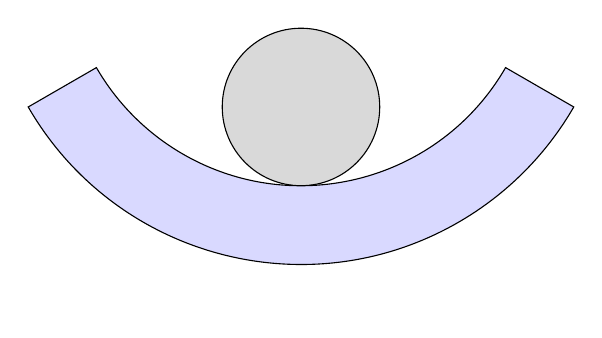
\begin{tikzpicture}
\filldraw [fill=gray!30, draw=black] (0,0) circle[radius=1];
\filldraw[fill=blue!15, draw=black, shift={(0,2)}] (330:3) arc (330:210:3) -- (210:4) arc (210:330:4) -- cycle;
\end{tikzpicture}

\end{tabular}

\end{document}